\documentclass[12pt,fleqn]{article}\usepackage{../../common}
\begin{document}
Temel Fizik 4 - Atalet Matrisi (Inertia Matrix, Tensor)

Bir objenin havaya fırlatıldığını düşünelim, fırlatma sırasında dönüş te var,
çetrefil bir hareket sözkonusu yani. Fakat şimdiye kadar gördüğümüz teknikler
ile hala bu hareketi analiz edebiliriz, hem lineer momentum, hem de açısal
momentum kütle merkezi odaklı olarak analiz edilebiliyor. Herhangi bir katı
gövde, cisim şeklini ve hareketi analiz için şimdi bazı genel formülleri
ortaya koyalım. 

Gövdenin açısal momentumu $L$ için [1, sf. 379],

$$
L = \sum m_i r_i \times v_i
$$

ki $L,r,v$ vektör. $v = \omega \times r$ eşitliğini üste sokarsak,

$$
L = \sum m_i r_i \times (\omega \times r_i)
\mlabel{1}
$$

Şimdi bu son ifadenin her vektörü öğelerini kullanarak açılımını yapalım böylece
başka bir forma erişmeyi umuyoruz. $\omega = [\begin{array}{ccc} \omega_x&\omega_y&\omega_z \end{array}]^T$
ve $r = [\begin{array}{ccc} x&y&z \end{array}]^T$ öğelerini kullanacağız, ve
üstteki formülün $A \times (B \times C)$ formunda olduğunu farkediyoruz, o zaman
genel bir $r \times (\omega \times r)$ üzerinde BAC-CAB açılımı yapmayı
deneyebiliriz, bu açılım hatırlarsak,

$$
A \times (B \times C) = B(A \cdot C) - C(A \cdot B)
$$

idi. Kendi denklemimiz üzerinde bu açılım

$$
r \times (\omega \times r) = \omega (r \cdot r) - r(r \cdot \omega)
$$

şeklinde olacaktır. Açılımı yapınca 3 x 1 boyutunda bir vektör elde ediyoruz
onun sadece ilk öğesine, $x$ için olan durumuna bakalım,

$$
r \times (\omega \times r)_x = \omega_x (x^2 + y^2 + z^2) - x(\omega_x x + \omega_y y + \omega_z z)
$$

$\omega_x x^2$ iki yerden iptal olur, kalanlar,

$$
 = \omega_x ( y^2 + z^2) - \omega_y xy + \omega_z xz
$$

Her üç öğe için açılım yapınca,

$$
r \times (\omega \times r) =
\left[\begin{array}{c}
(y^2 + z^2) \omega_x - xy \omega_y - xz \omega_z \\
-yx \omega_x + (z^2 + x^2)\omega_y - yz \omega_z \\    
-zx \omega_x - zy \omega_y + (x^2+y^2)\omega_z
\end{array}\right]
$$

Ve ana formülde $m_i$ çarpımı olduğunu unutmayalım,

$$
m r \times (\omega \times r) =
\left[\begin{array}{c}
m (y^2 + z^2) \omega_x - m xy \omega_y - m xz \omega_z \\
-m yx \omega_x + m (z^2 + x^2)\omega_y - m yz \omega_z \\    
-m zx \omega_x - m zy \omega_y + m (x^2+y^2)\omega_z
\end{array}\right]
$$

Ustteki sonucu (1)'e sokunca, ve notasyonel olarak bazı rahatlıklar düşünerek,
mesela $I_{xx} = \sum_i m_i (y_i^2 + z_i^2)$ gibi, ya da $I_{xy} = - \sum_i m x_i y_i$.
Bunları da yerine koyunca, $L_x,L_y,L_y$ diyelim,

$$
L_x = I_{xx} \omega_x + I_{xy} \omega_y + I_{xz} \omega_z
$$

$$
L_y = I_{yx} \omega_x + I_{yy} \omega_y + I_{yz} \omega_z
$$

$$
L_z = I_{zx} \omega_x + I_{zy} \omega_y + I_{zz} \omega_z
$$

Fakat bu son sonuç hala biraz sadeleştirilebilir. İfadeye bakarsak onu bir
matris çarpı bir vektör çarpımı ile temsil edebiliriz gibi geliyor,
hakikaten de

$$
I = \left[\begin{array}{ccc}
I_{xx} & I_{xy} & I_{xz} \\
I_{yx} & I_{yy} & I_{yz} \\
I_{zx} & I_{zy} & I_{zz} 
\end{array}\right], \quad
\omega = \left[\begin{array}{c}
\omega_x \\ \omega_y \\ \omega_z
\end{array}\right]
$$

üzerinden $I \omega$ çarpımının (2) sonucunu vereceğini görebiliriz. Böylece
gayet sade

$$
L = I \omega
$$

ifadesine geri gelmiş olduk.

$I$, atalet matrisidir, ve her katı kütle şekline göre farklı olacak bir
matristir. O zaman bir objenin açısal momentumunun nasıl olacağını hesaplamak
için önce o objenin atalet matrisine hesaplamak gerekir.

Ataletin Ana Eksenleri (Principal Axes of Inertia) 

Bir konu daha var tabii; dikkat edersek $I$ matrisini çekip çıkardığımız hesap
bir $O$ referansını merkez alıyordu. ``Genel bir $O$ olsun'' dedik ve oradan
türetmeye devam ettik. Fakat bazı referansların, yani dönüşün neyin etrafında
olduğunun, her seçime göre farklı $I$'lara sebebiyet verebileceğini görmek
gerekir. Lineer cebirsel olarak $L$ ile $\omega$'nin aynı yönü göstermesi için
$I$'nin köşegen matris olması gerekir. Fakat elde köşegen matris olmasa da
$\omega$'yi bizim değiştirerek, aynı refarans $O$'dan geçen ama farklı öyle bir
yönü göstermektir ki, bu eksen etrafında bir köşegen $I$ elde edilsin ve hareket
simetrik hale gelsin.

Bu hesap icin ozdeger, ozvektor hesabini yapmak lazim, ya da atalet matrisinin
kosegenlestirilmesini [2] (diagonalization) gerceklestirmek lazim. Eger $I$
kosegen degil ise, oyle bir $\omega$ bulalim ki $L = I \omega$ hesabindaki
$L$, $I \omega$ ile ayni yonu gostersin, yani

$$
I\omega = \lambda \omega
$$

haline gelsin. Bu bir özdeğer problemi değil midir? Evet. 

Örnek olarak [1, sf. 382]'deki $O$ etrafında dönen küp orneğini kullanalım,

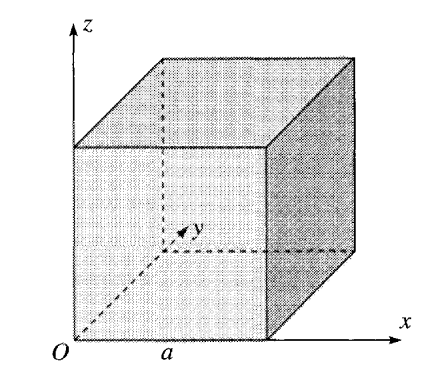
\includegraphics[width=20em]{phy_005_basics_04_01.png}

Bu referansa gore atalet matrisi

$$
I = \left[\begin{array}{rrr}
8 & -3 & -3 \\
-3 & 8 & -3 \\
-3 & -3 & 8
\end{array}\right]
$$

olarak bulunmuş. Görüldüğü gibi $I$ köşegen değil. Kosegenlestirmek icin,

\begin{minted}[fontsize=\footnotesize]{python}
import numpy.linalg as lin
I = np.array([[8, -3, -3],
              [-3, 8, -3],
              [-3, -3, 8]])
pe,lam = lin.eig(I)
print (e)
\end{minted}

\begin{verbatim}
[11.  2. 11.]
\end{verbatim}

Demek ki yeni $I$ matrisi

$$
I = \left[\begin{array}{rrr}
11 & 0 & 0 \\
0 & 2 & 0 \\
0 & 0 & 11 
\end{array}\right]
$$

olmalı.

[devam edecek]

Kaynaklar

[1] Taylor, {\em Classical Mechanics}

[2] Bayramli, {\em Lineer Cebir, Ders 22}

\end{document}
